\documentclass[letterpaper,12pt]{article}

\usepackage{threeparttable}
\usepackage{geometry}
\geometry{letterpaper,tmargin=1in,bmargin=1in,lmargin=1.0in,rmargin=1.0in}
\usepackage[format=hang,font=normalsize,labelfont=bf]{caption}
\usepackage{amsmath}
\usepackage{multirow}
\usepackage{array}
\usepackage{delarray}
\usepackage{amssymb}
\usepackage{amsthm}
\usepackage{lscape}
\usepackage{natbib}
\usepackage{setspace}
\usepackage{float,color}
\usepackage[pdftex]{graphicx}
\usepackage{listings}
\lstset{basicstyle=\footnotesize\ttfamily, language=Python, showstringspaces=false}

\lstset{frame=single,
  language=Python,
  showstringspaces=false,
  columns=flexible,
  basicstyle={\small\ttfamily},
  numbers=none,
  breaklines=true,
  breakatwhitespace=true
  tabsize=3
}

\usepackage{pdfsync}
\usepackage{booktabs}
\usepackage{verbatim}
\usepackage{placeins}
\usepackage{geometry}
\usepackage{pdflscape}
\synctex=1
\usepackage{hyperref}
\hypersetup{colorlinks,linkcolor=red,urlcolor=blue,citecolor=red}
\usepackage{bm}


\theoremstyle{definition}
\newtheorem{theorem}{Theorem}
\newtheorem{acknowledgement}[theorem]{Acknowledgement}
\newtheorem{algorithm}[theorem]{Algorithm}
\newtheorem{axiom}[theorem]{Axiom}
\newtheorem{case}[theorem]{Case}
\newtheorem{claim}[theorem]{Claim}
\newtheorem{conclusion}[theorem]{Conclusion}
\newtheorem{condition}[theorem]{Condition}
\newtheorem{conjecture}[theorem]{Conjecture}
\newtheorem{corollary}[theorem]{Corollary}
\newtheorem{criterion}[theorem]{Criterion}
\newtheorem{definition}{Definition}  % Number definitions on their own
\newtheorem{derivation}{Derivation}  % Number derivations on their own
\newtheorem{example}[theorem]{Example}
\newtheorem{exercise}[theorem]{Exercise}
\newtheorem{lemma}[theorem]{Lemma}
\newtheorem{notation}[theorem]{Notation}
\newtheorem{problem}[theorem]{Problem}
\newtheorem{proposition}{Proposition}  % Number propositions on their own
\newtheorem*{proposition*}{Proposition}  % Non-numbered proposition
\newtheorem{remark}[theorem]{Remark}
\newtheorem{solution}[theorem]{Solution}
\newtheorem{summary}[theorem]{Summary}
\bibliographystyle{aer}
\newcommand\ve{\varepsilon}
%\renewcommand\theenumi{\roman{enumi}}
\newcommand\norm[1]{\left\lVert#1\right\rVert}

\begin{document}

\begin{titlepage}
\title{The Economic Costs of a Resurgence of Disease in South Africa}
\date{March 2025}
\author{\href{http://jasondebacker.com/}{Jason DeBacker}\thanks{University of South Carolina, Darla Moore School of Business, Department of Economics, \href{mailto:jason.debacker@moore.sc.edu}{jason.debacker@moore.sc.edu}. All Python code and documentation for the computational examples and analyses are available at \href{https://github.com/OpenSourceEcon/CostOfDisease}{https://github.com/OpenSourceEcon/CostOfDisease}.}\and \href{https://sites.google.com/site/rickecon}{Richard W. Evans}\thanks{\href{https://abundance.institute/}{Abundance Institute}, \href{mailto:rick@abundance.institute}{rick@abundance.institute}.}\and Marcelo T. LaFleur\thanks{United Nations Department of Economic Social Affairs}, \href{mailto:lafleurm@un.org}{lafleurm@un.org}.}
\maketitle
\vspace{-2mm}
\begin{abstract}
\small{Reductions in U.S. foreign aid are expected to have significant public health impacts.  We estimate the economic costs of these reductions in terms of lost health and productivity for South Africa.  We find that the reductions in foreign aid and expected significant increases in disease and premature death, will have very large and negative impacts on the South African economy.  In our preferred specification, the costs exceed XX trillion rand (about \$X trillion dollars) in net present value.}

\vspace{10mm}

\noindent\textit{keywords:}\: public health, demographics, general equilibrium, productivity, South Africa

\vspace{10mm}

\noindent\textit{JEL classification:} C68, E24, E37, I15, J11, J17, J24


\end{abstract}
\thispagestyle{empty}
\end{titlepage}


\begin{spacing}{1.5}

\pagenumbering{arabic}

\newpage

\section{Introduction}\label{SecIntro}

South Africa has carried one of the world’s heaviest HIV/AIDS burdens for over two decades. HIV prevalence has remained among the highest globally, with 17.1\% of adults infected with the virus in 2023 and a total of 7.7 million people living with HIV \citep{UNAIDSData2024}. The dual burden of HIV and tuberculosis (TB)—still the world’s deadliest infectious disease—has compounded the country’s health crisis. 

This persistent disease burden has generated far-reaching economic and social consequences. As of 2023, 5.9 million people between the ages of 15 and 49 were HIV-positive, and South Africa recorded the highest absolute labor income losses globally due to HIV-related illness and mortality \citep{ILO2018}. These effects are not confined to the formal labor market: unpaid care burdens, disruptions to education, and lower household productivity compound the long-term developmental cost. The cumulative strain on human capital, social protection systems, and economic growth has become a defining feature of South Africa’s development trajectory.

Despite these challenges, the large-scale expansion of antiretroviral therapy (ART) has dramatically improved survival and reduced transmission. By 2023, approximately 77\% of HIV-positive individuals were receiving ART, reflecting one of the highest coverage rates in the region \citep{UNAIDSData2024}. This progress was made possible largely through sustained external financing and partnerships that supported clinical infrastructure, drug procurement, and health workforce training. South Africa’s response to HIV and TB has thus become structurally dependent on international support. Continued access to external funding has been essential to maintaining treatment programs, expanding prevention efforts, and preserving health system resilience. 

However, this reliance also introduces vulnerabilities in the face of shifting global aid priorities—especially given the outsized role of the United States in financing HIV/AIDS programs in low- and middle-income countries, particularly through the President’s Emergency Plan for AIDS Relief (PEPFAR). According to the \citet{FGH2023} report, total U.S. development assistance for health (DAH) rose from \$19.1 billion in 2021 to approximately \$20.6 billion in 2023—a 7.8\% increase. Funding for HIV/AIDS accounted for nearly \$8.6 billion of that total in 2023. South Africa is among the largest absolute recipients of this assistance, receiving funding that supports prevention programs, treatment coverage, public health infrastructure, and the training of medical personnel. Though countries such as Eswatini and Lesotho receive more funding per capita, the scale of South Africa’s epidemic and population has made U.S. support an indispensable foundation of its national HIV response.

In early 2025, the U.S. government abruptly halted all USAID health disbursements, terminating more than 5,800 (out of 6,300) contracts and grants globally in previously obligated commitments \citep{Cohen2025}. The fallout was immediate: UNAIDS lost nearly half its budget, clinics suspended services, and millions faced interruptions in care. In South Africa, public health leaders warned of a collapse in ART delivery systems, re-emergence of opportunistic infections, and surges in preventable deaths. The World Health Organization simultaneously issued an alert on disruptions to TB services, calling for urgent global action.

The human toll of this withdrawal is projected to be devastating. \citet{KS2025} estimate that the complete elimination of U.S. global health funding could result in as many as 3.3 million excess deaths worldwide each year, with HIV/AIDS accounting for the majority of these losses. \citet{Gandhi2025} estimate that the cessation of PEPFAR funding could lead to up to 2.9 million additional HIV-related deaths over a ten-year period under the most severe scenario. \Citet{Brink2025} estimate in the worst case scenario that as many as 2.9 million people could die from HIV/AIDS in low- and middle-income countries over the next five years. 

For South Africa, the various sources estimate excess deaths from HIV alone could amount anywhere from 14,000 to 192,000 annually, depending on the scenario. In addition to the direct loss of life, the increased disease burden resulting from disrupted treatment is expected to increase absenteeism and reduce labor productivity. These illness-related work absences can significantly lower effective labor supply \citep{Keogh2024,Panda2024}. These estimates highlight the scale of the crisis and provide the basis for our economic simulation.

We estimate the macroeconomic impact of this aid withdrawal using an overlapping generations (OG) model calibrated for South Africa. We use the mortality scenarios derived from recent projections by \citet{KS2025} and by \citet{Gandhi2025} and expected changes to labor productivity associated with the higher disease burden \citep{Keogh2024,Panda2024}. In our framework, higher mortality and increased illness-related disutility of labor lead to reductions in labor supply, human capital, and long-run output. Scenarios range from a ``Resilient'' response in which the health system partially absorbs the shock, to a ``Susceptible'' case in which mortality surges by 84\% relative to the baseline. 

By evaluating these scenarios, this paper contributes to understanding the long-run economic costs of disease and the structural fragility of health systems that are highly dependent on external financing. The findings highlight not only the human toll of abrupt aid cessation but also its deep implications for macroeconomic performance and national development.


\section{Methodology}\label{SecMethod}

We use the OG-ZAF model (cite it) to estimate the economic costs of a resurgence of disease in South Africa.  The model is a dynamic, general equilibrium model that includes a detailed representation of the South African economy, including its demographics, health, and productivity.  The model is calibrated to match the South African data and is used to simulate the economic impacts of a resurgence of disease in South Africa.

\textbf{Give brief overview of model, but omit equations etc in main text.  Cite OG-Core as well as OG-ZAF (and footnote with links to docs for details).}

This paper evaluates the long-run macroeconomic effects of an abrupt reduction in U.S. bilateral HIV funding to South Africa. Our analysis integrates a range of epidemiological projections into a dynamic overlapping generations model of the South African economy. The model simulates the estimated changes in population structure and productivity in response to the sudden stop in external aid, allowing us to quantify the aggregate and distributional economic effects of increased mortality and morbidity due to disruptions in HIV programming.

\subsection{Epidemiological Scenarios}
We use the clinical and economic projections from \citet{KS2025}, \citet{Gandhi2025}, and \citet{Brink2025}. 

\citet{KS2025} estimate the lives saved by U.S. foreign aid through both gross and net approaches. For HIV/AIDS, their gross estimate is based on the number of individuals receiving PEPFAR-funded antiretroviral therapy, combined with survival rates for untreated HIV to calculate an annualized total of 1.6 million lives saved (though the authors suggest this estimate is biased by the presence of small countries with high HIV prevalence). Their net estimate relies on a differences-in-differences analysis which compares adult mortality trends in PEPFAR focus countries to non-PEPFAR recipient control countries. This analysis suggests that PEPFAR reduced all-cause mortality by roughly three deaths per 1,000 adults annually. Applying this to total U.S. global HIV/AIDS aid yields an upper-bound estimate of nearly 3 million deaths averted per year, though the authors note this may overstate the true effect. For South Africa the authors estimate that 192,212 lives are saved each year due to US funding, and this is used as the upper-bound of expected lives lost due to the cancellation of US health aid. 

\citet{Gandhi2025} model clinical and economic outcomes under three scenarios of PEPFAR funding in 2024: full support, partial support, and complete withdrawal. Using the CEPAC-International microsimulation model,\footnote{https://mpec.massgeneral.org/cepac-model} they project changes in HIV incidence, treatment coverage, and AIDS-related mortality in South Africa. The model tracks disease progression, care engagement, and mortality for both people with HIV and those at risk. Importantly, they also consider the effects of funding cuts on testing capacity, re-engagement in care, and prevention services. Under a scenario of complete withdrawal, the model estimates as many as 1.3 million excess deaths over ten years in South Africa, relative to full funding.

\Citet{Brink2025} estimate the expected increase in HIV-related mortality across 36 PEPFAR-supported countries by combining funding reduction scenarios with empirical elasticities derived from historical changes in treatment coverage and mortality. Their results show a sharp gradient in cumulative excess deaths from 2025 to 2030, depending on the scenario. In more benign scenarios there are few additional deaths. In more severe scenarios, where PEPFAR is discontinued, the projected excess mortality over the five-year period reaches 282,950 with mitigation efforts, and 491,750 without mitigation—averaging 56,590 and 98,350 additional deaths per year, respectively.

\subsection{Absenteeism and productivity scenarios}
To simulate the economic impact of disease-related morbidity among working-age individuals, we impose an adjustment that reflect the effects of untreated or poorly managed HIV and tuberculosis which totals 0.4\% each year. These are implemented as adjustments to the labor disutility parameter, applied to the bottom 70\% of ability types among working-age individuals (ages 20–64) in the reform policy simulation. This is implemented as changes to the $\chi_n$ matrix (disutility of labor) and held constant to reflect persistent productivity losses in the absence of expanded care.

\textbf{HIV-related productivity shock.}: The HIV-related productivity shock is grounded in the ILO’s global estimates of the economic impact of AIDS, which quantify those that are partially or fully unable to work \citet{ILO2018}. Historical data for South Africa from 2005 to 2020 show a sharp decline in the number of individuals partially or fully unable to work—from over 163,000 in 2005 to fewer than 2,300 in 2020—due to improved access to ART and labor market inclusion. To simulate a reversal of these gains under scenarios of reduced HIV service coverage (e.g., PEPFAR withdrawal), we assume a return to earlier levels of absenteeism. We use the ILO’s “high” scenario to estimate the degree of absenteeism of those partially unable to work, the historical shares of those fully unable to work, and the projected HIV prevalence in the labor force (23.9\%) to estimate the total absenteeism from 2025 to 2040. For the worst-case scenario we use the full impact by 2040 as the immediate and constant effect. 

\textbf{TB-related productivity shock.}: For tuberculosis, we apply an additional uniform productivity penalty of 0.00027581, based on South Africa’s 2023 TB incidence by age and empirical estimates of lost workdays. The estimate assumes a high-impact scenario of 0.1442\% absenteeism loss per TB case, reflecting reduced access to diagnosis and treatment. This is applied to the prevalence of TB in the working age population and held constant over time.



% figure
\begin{figure}[h]
    \caption{Mortality rates with and without aid}
    \centering
    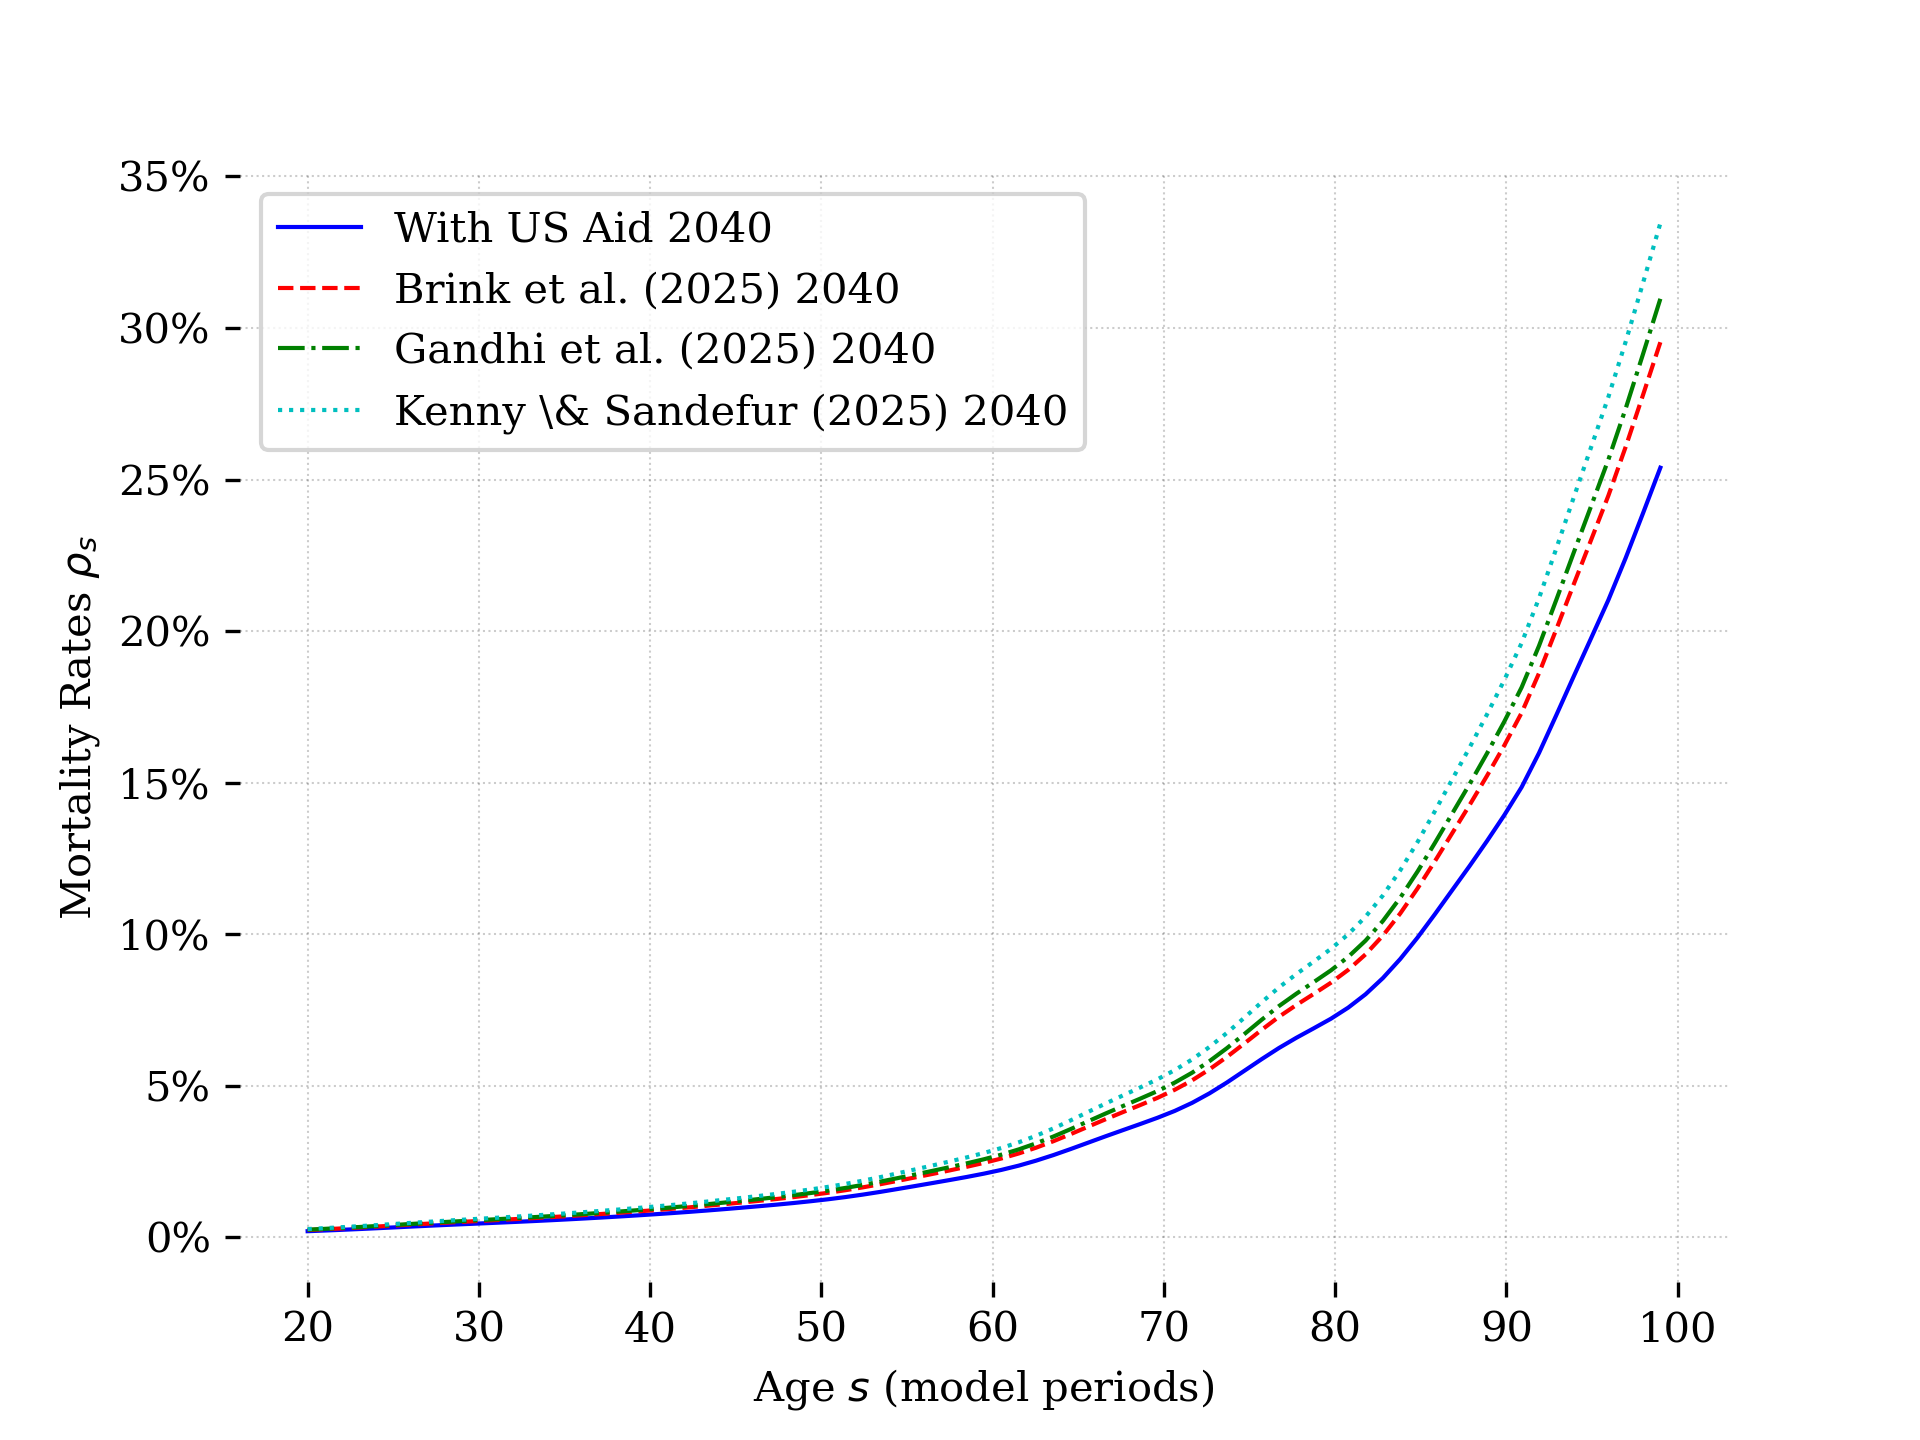
\includegraphics[scale=0.75]{./tables_figures/mortality_rates.png}
\end{figure}

The population distribution is affected by the changes in mortality rates:
\begin{figure}[h]
    \caption{The population distribution with and without aid}
    \centering
    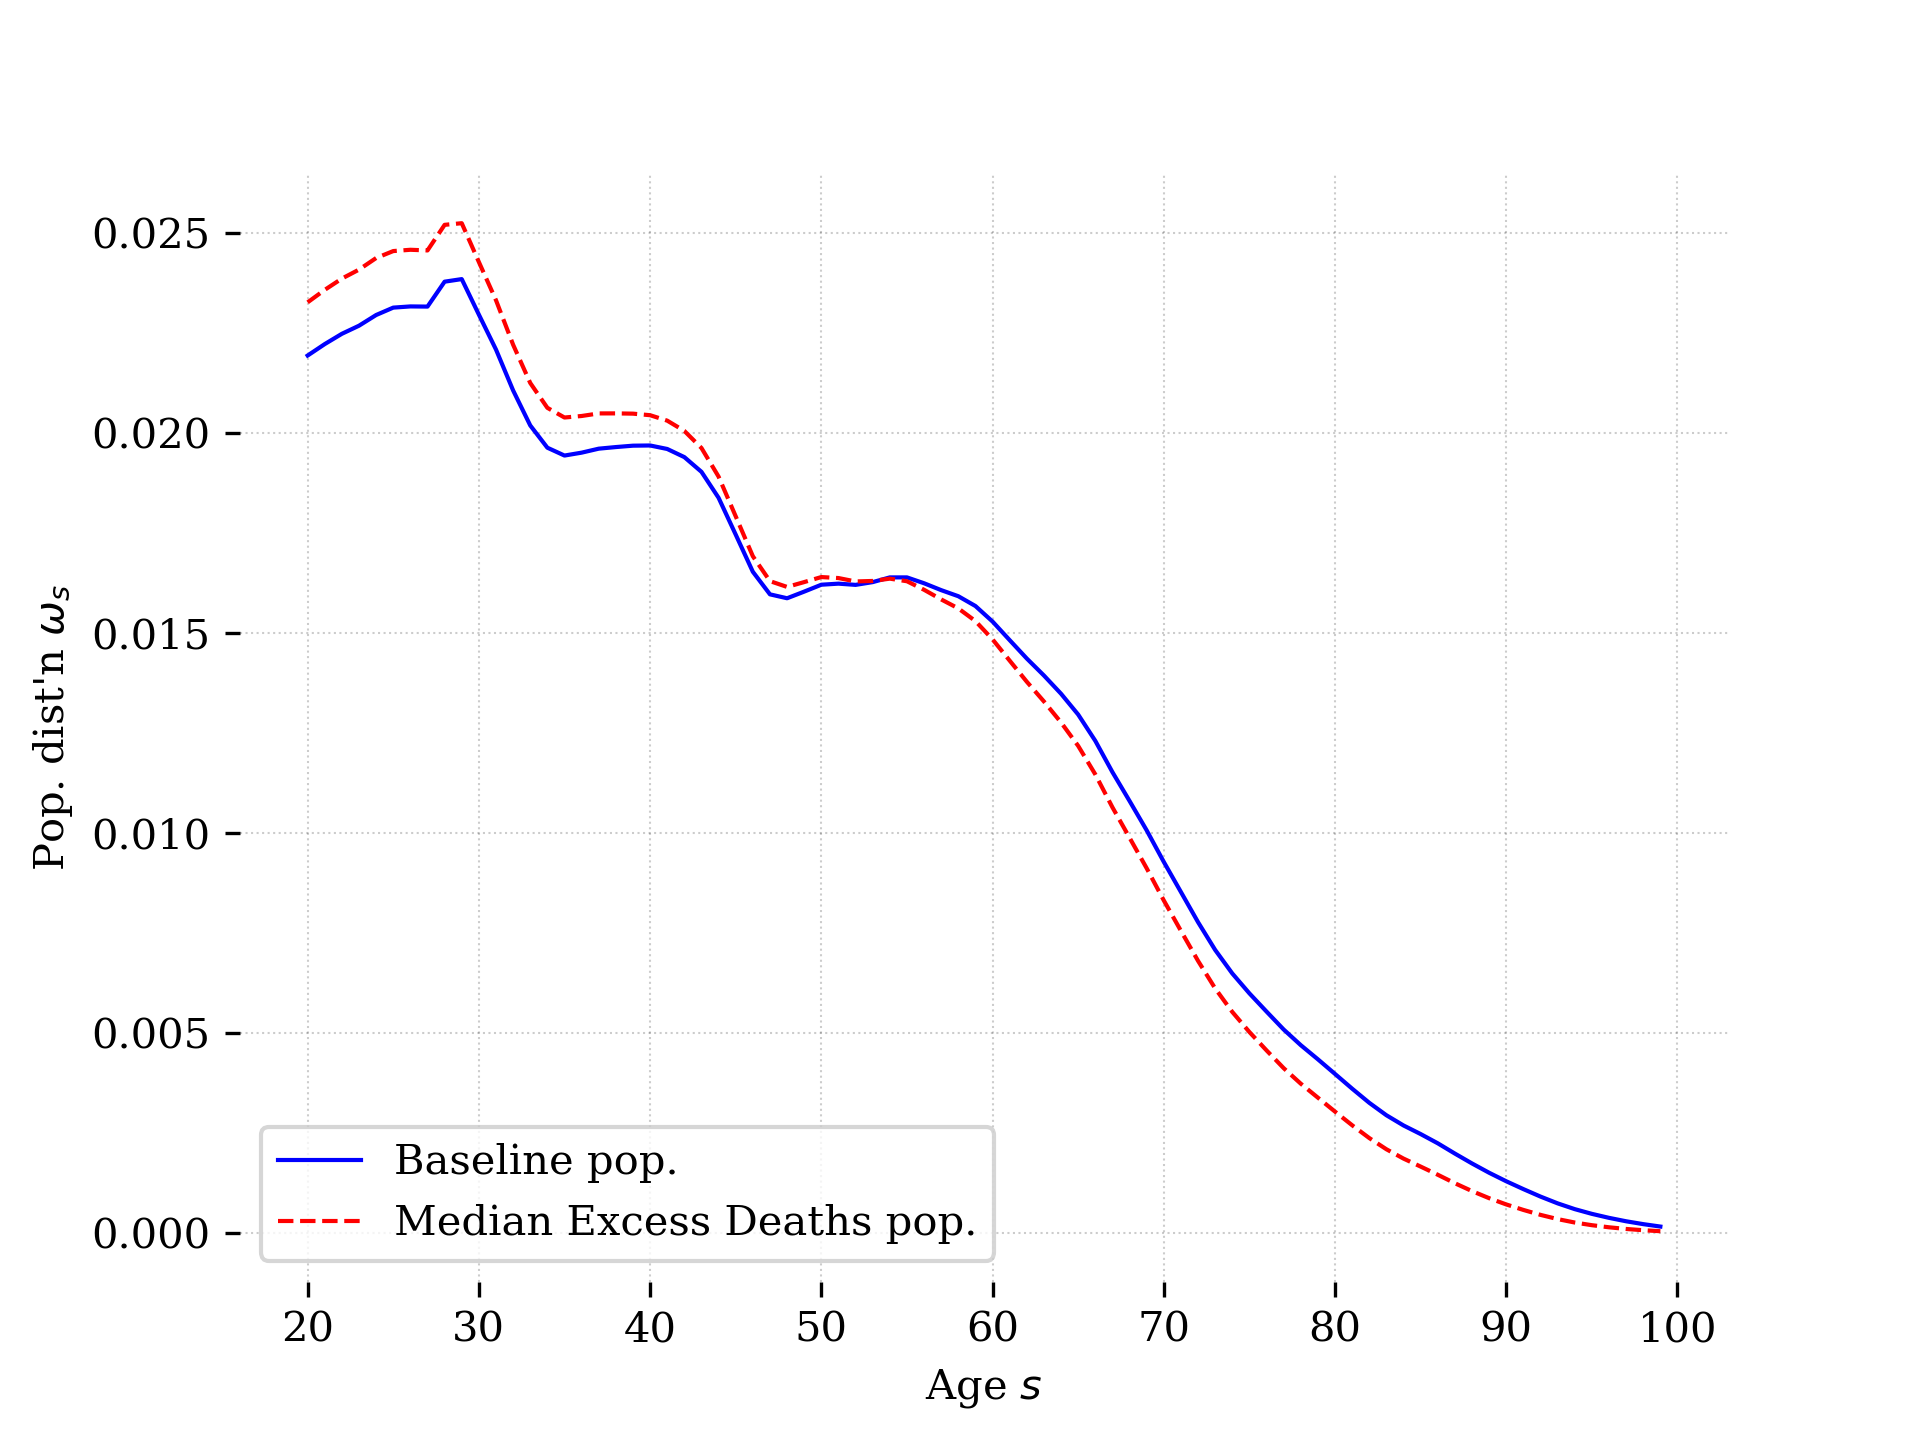
\includegraphics[scale=0.75]{./tables_figures/pop_dist_2050.png}
\end{figure}

TODO: create and add a figure here with cumulative deaths.

Describe how we incorporate productivity effects into the model (cite that research):

\begin{figure}[h]
    \caption{Labor productivity with and without aid}
    \centering
    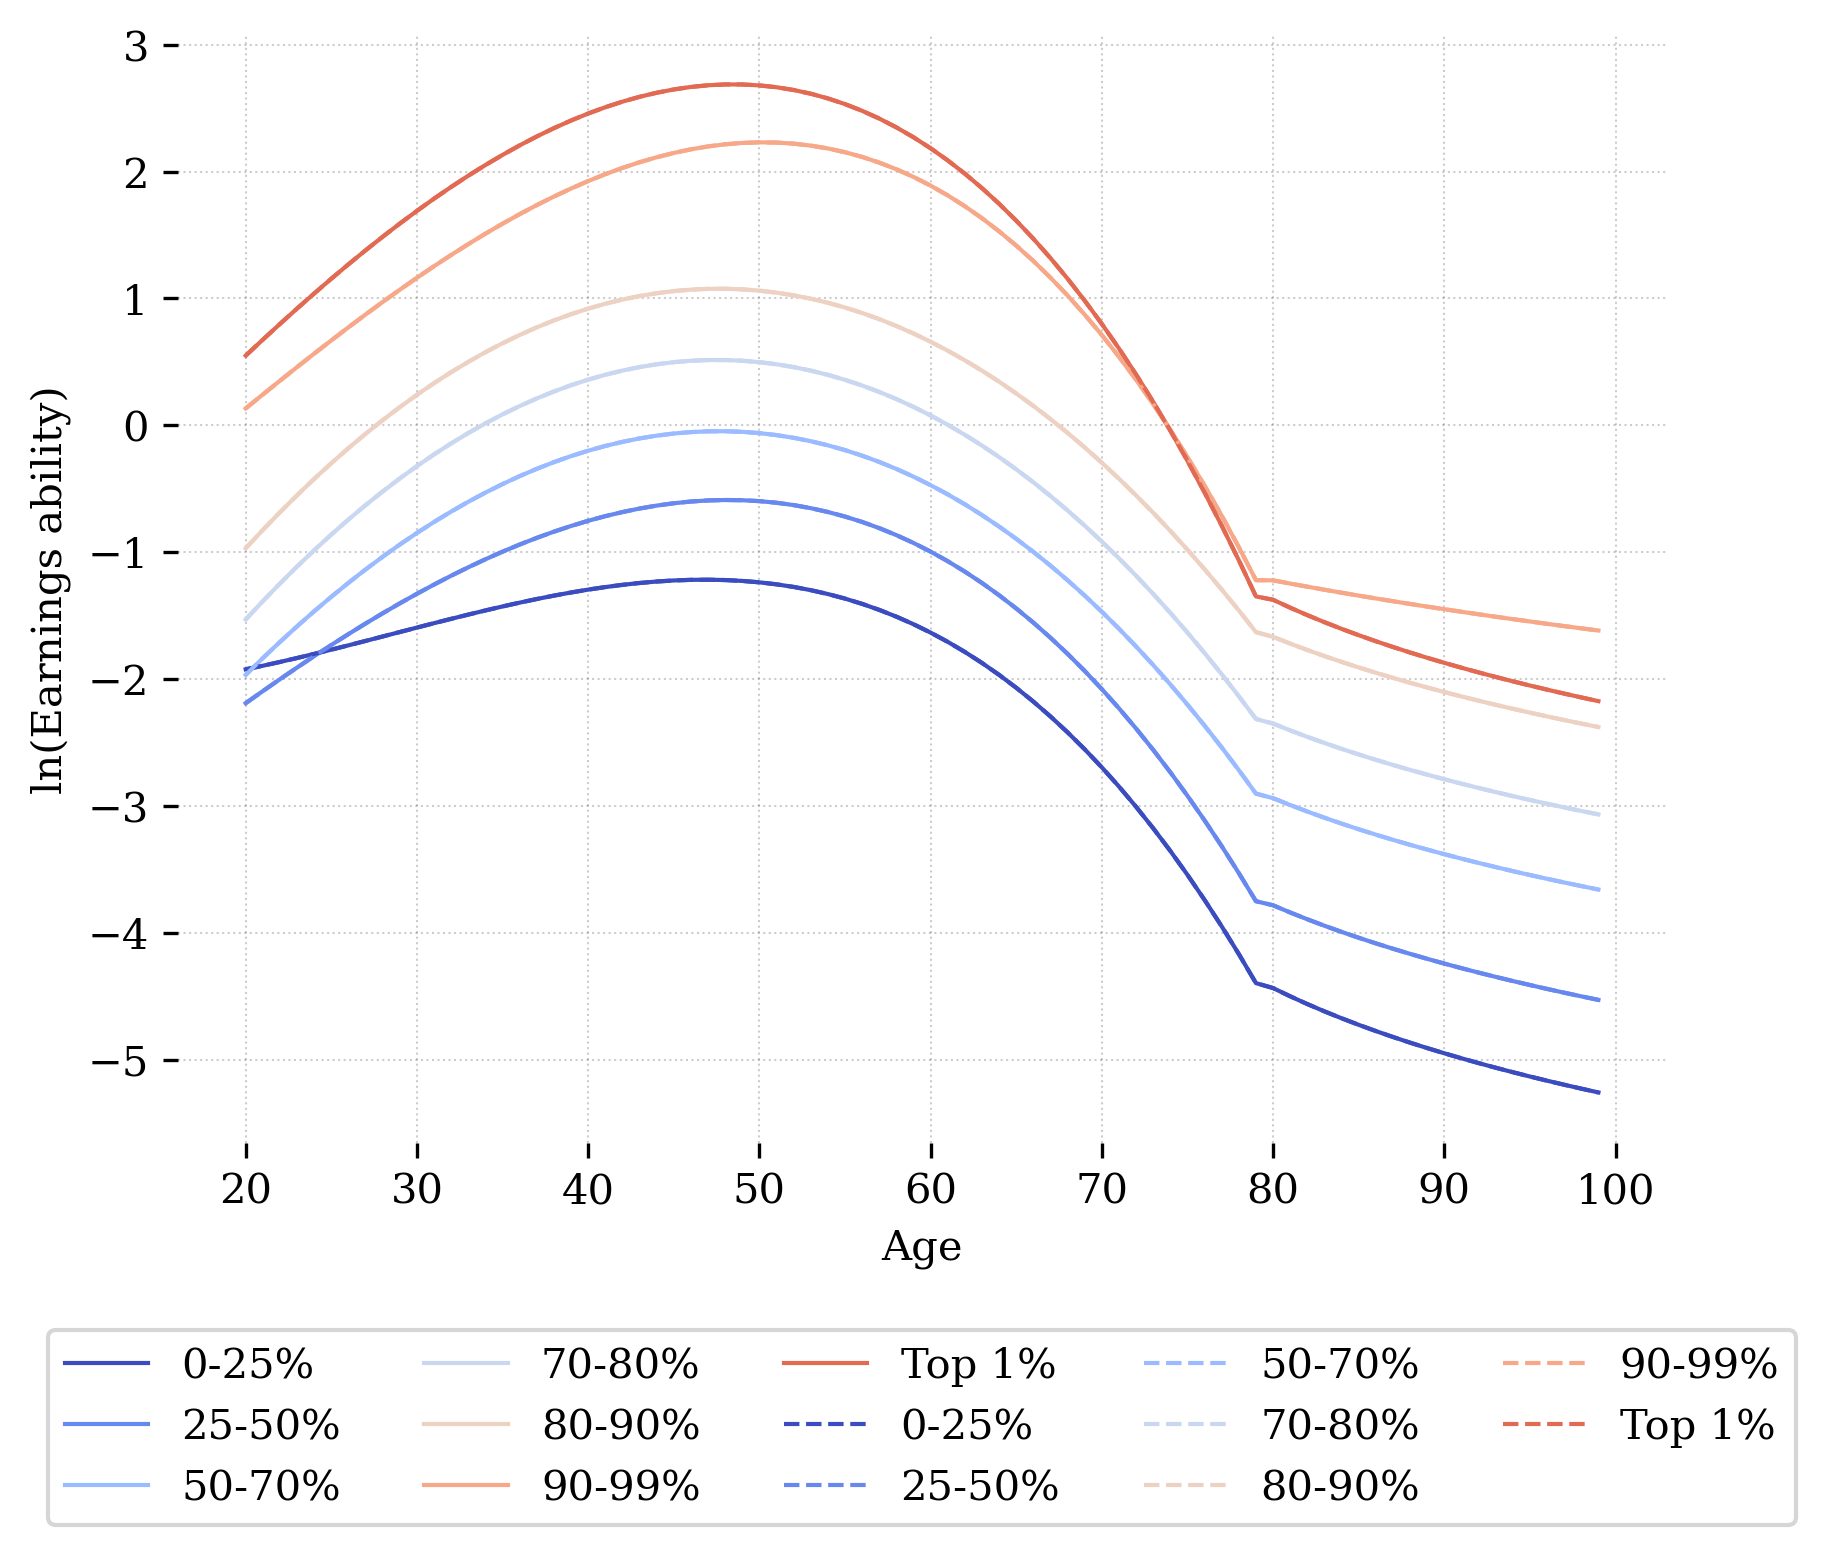
\includegraphics[scale=0.75]{./tables_figures/ability_profiles.png}
\end{figure}

\section{The Economics Costs of Disease}\label{SecResults}

We find that the economic costs of a resurgence of disease in South Africa are very large.  In our preferred specification, the costs exceed XX trillion rand (about \$X trillion dollars) in net present value.  The costs are driven by the large increases in mortality rates and the resulting reductions in labor productivity.

Put in tables and figures showing: Changes in GDP over first few years, NPV of effect, plot of cumulative deaths (or number of people).

Trillions per year. average over 20 years.
\begin{tabular}{lr}
\toprule
 & $\Delta$ GDP, Trillions \\
\midrule
Low Excess Deaths & -0.01 \\
Median Excess Deaths & -0.02 \\
High Excess Deaths & -0.02 \\
\bottomrule
\end{tabular}


NPV in trillions
\begin{tabular}{rlrrr}
\toprule
index & Discount Rate & Low Excess Deaths & Median Excess Deaths & High Excess Deaths \\
\midrule
0 & 2\% & -0.42 & -2.27 & -3.99 \\
1 & 4\% & -0.30 & -0.91 & -1.49 \\
2 & 6\% & -0.19 & -0.45 & -0.71 \\
\bottomrule
\end{tabular}


Have some robustness by looking at high and low values of the forecast of excess deaths/effects on productivity.

\section{Conclusion}\label{SecConc}

Sum up what we said.  Compare economic costs to the amount of aid that is at stake.

\end{spacing}
\newpage
\bibliography{disease.bib}


\end{document}